\documentclass[UTF8,AutoFakeBold,AutoFakeSlant,zihao=-4]{ctexart}

\newcommand{\emp}{\noindent\fboxsep=0pt}

\usepackage{wrapfig}
\usepackage{fontspec}
\usepackage{color}
\usepackage{fancyhdr}
\usepackage{setspace}
\usepackage{caption}
\usepackage{mathptmx}
\usepackage{amsmath}
\usepackage{amssymb}
\usepackage{amstext}
\usepackage{geometry}
\usepackage{graphicx}
\usepackage{enumerate}
\usepackage{enumitem}
\usepackage{pifont}
\usepackage{float}
\usepackage{newclude}
\usepackage{subfig}
\usepackage{multirow}
\usepackage{tabularx}
\geometry{
a4paper,
left=2.5cm,
right=2.5cm,
top=2.5cm,
bottom=2.5cm,
}
%\usepackage{listings}
%\usepackage{boxedminipage}

% 设置n倍行距(需要注释掉正文中设置行距的部分)
% \linespread{1.5} % 正文1.5倍行距

%定义一级二级三级标题
\ctexset{
	section = {	% 定义一级标题 
	           	format+ = \zihao{4} \heiti \raggedright, 	% 字号为’四号‘,字体为’黑体‘,左对齐
	           	name = {,、},                             	% 序号后面加’、‘
	           	number = \chinese{section},              	% 序号为’汉字‘
	           	beforeskip = 1.0ex plus 0.2ex minus .2ex,	% 标题前的垂直间距 = 基础高度为1.0ex,可以伸展到 1.0 - 0.2 = 1.2ex,也可以收缩到 1.0 - .2 = 0.8ex; ex为当前字号下字母x的高度
	           	afterskip = 1.0ex plus 0.2ex minus .2ex, 	% 标题后的垂直间距 = ...	
	           	aftername = \hspace{0pt}                 	% 编号和标题之间的格式 = 增加水平间距’0pt‘ 
	},
	subsection = {	% 定义二级标题
	              	format+ = \zihao{-4} \songti \raggedright,
	              	name = {(,)},
	              	number = \chinese{subsection},	% 序号为’阿拉伯数字‘
	              	beforeskip = 1.0ex plus 0.2ex minus .2ex,
	              	afterskip = 1.0ex plus 0.2ex minus .2ex,
	              	aftername = \hspace{0pt},
	},
	subsubsection = {
			format+ = \zihao{-4} \songti \raggedright,
			name = {\qquad,\ \enspace},
			number = {\arabic{section}.\arabic{subsection}.\arabic{subsubsection}},	
			beforeskip = 1.0ex plus 0.2ex minus .2ex,
			afterskip = 1.0ex plus 0.2ex minus .2ex,
			aftername = \hspace{0pt},
	}
}

% 设置页眉页码
\pagestyle{plain} % 取消页眉
\lfoot{}	% 页码出现在下方

% 定义正文字体
\setromanfont{Times New Roman}	% 将西文字体设置为 Times New Roman
% \setCJKfamilyfont{zhkai}{[SIMKAI.TTF]}
% \newcommand*{\kaiti}{\CJKfamily{zhkai}}

% 定义 caption
\DeclareCaptionFont{kaiticaption}{\kaishu \small}	% 定义下面三个caption的font的kaiticaption的具体格式
\captionsetup[figure]{font=small,labelsep=quad,skip=0.5ex,labelfont=bf,font=kaiticaption}	% 设置图片的 caption 格式 % 想要标题换行后居中,可以添加justification=centering
\captionsetup[table]{font=small,labelsep=quad,skip=0.5ex,labelfont=bf,font=kaiticaption}	% 设置表格的 caption 格式
\captionsetup[subfloat]{font=small,labelsep=quad,skip=0.5ex,labelfont=bf,font=kaiticaption}
\captionsetup[equation]{font=small,labelsep=quad,skip=0.5ex,labelfont=bf,font=kaiticaption}


% 设置图片,表格,公式编号格式
\renewcommand{\thetable}{\thesection{}-\arabic{table}}	% \thetable 表示设置的是表格的编号格式, 后面括号的内容为编号格式:章节号-表格的序号
\renewcommand{\thefigure}{\thesection{}-\arabic{figure}}
\renewcommand{\theequation}{\thesection{}-\arabic{equation}}

% 设置列表标签
\setlist[enumerate]{nosep,itemindent=0.75em,labelsep=0.5em}	% labelsep 是标签与标签后面内容的间距(这里是一个空格),leftmargin是标签后面内容与左边界之间的距离
\setlist[itemize]{nosep,itemindent=0.5em, labelsep=0.5em}
\setlist[description]{nosep,leftmargin=*}
\let\olddescriptionlabel\descriptionlabel  
\renewcommand{\descriptionlabel}[1]{\hspace{2em}\olddescriptionlabel{#1}:}  


% 设置代码块
%\definecolor{commentcolor}{RGB}{85,139,78}
%\definecolor{stringcolor}{RGB}{206,145,108}
%\definecolor{keywordcolor}{RGB}{34,34,250}
%\lstset{
%	language=Matlab, % 默认代码语言.
%	basicstyle=\footnotesize,
%	numbers=left, %设置行号位置
%	numberstyle=\tiny, %设置行号大小
%	commentstyle=\color{commentcolor},	%注释颜色
%	keywordstyle=\color{keywordcolor},	%关键词颜色
%	stringstyle=\color{stringcolor},	%字符串颜色
%	frame=single, %设置边框格式
%	escapeinside=``, %逃逸字符(1左面的键),用于显示中文
%	breaklines = True, % 自动折行
%	breakatwhitespace = True, % 自动折行时打断单词
%	extendedchars=false, %解决代码跨页时,章节标题,页眉等汉字不显示的问题
%	xleftmargin=2em,xrightmargin=2em, aboveskip=1em, %设置边距
%	tabsize=4, %设置tab空格数
%	showspaces=false %不显示空格
%}

\graphicspath{{../img/}}
\title{车身系统}
\author{}
\date{}
\begin{document}
\setlength{\parskip}{0em}	% 段前段后间距为 0
\setlength{\parindent}{2em} % 正文首行悬挂: 2汉字字符
\setlength{\baselineskip}{20pt}	% 正文行间距20磅
\selectfont	% 刷新行间距信息
\setlength{\lineskip}{10pt}		% 推荐设置为行距的一半
\setlength{\lineskiplimit}{10pt}	% 同上
\abovedisplayshortskip=0pt	%设置公式距离上方非重叠区域额外添加的距离,推荐0
\belowdisplayshortskip=0pt
\abovedisplayskip=0pt	%设置公式距离上方重叠距离额外添加的距离,推荐0
\belowdisplayskip=0pt
\renewcommand{\arraystretch}{1.5}

\maketitle
\section{车身概述}
车辆用来载人装货的部分
\subsection{分类(按是否带车架)}
	\begin{itemize}
		\item 非承载式车身
			\begin{itemize}
				\item 装备该非承载式车身的车辆有独立的车架,车身固定在车架上
				
				\item 质量大,高度高,一般用在越野车、皮卡车上
				
					\begin{figure}[htbp]
						\centering
						\caption*{车身及底盘}
						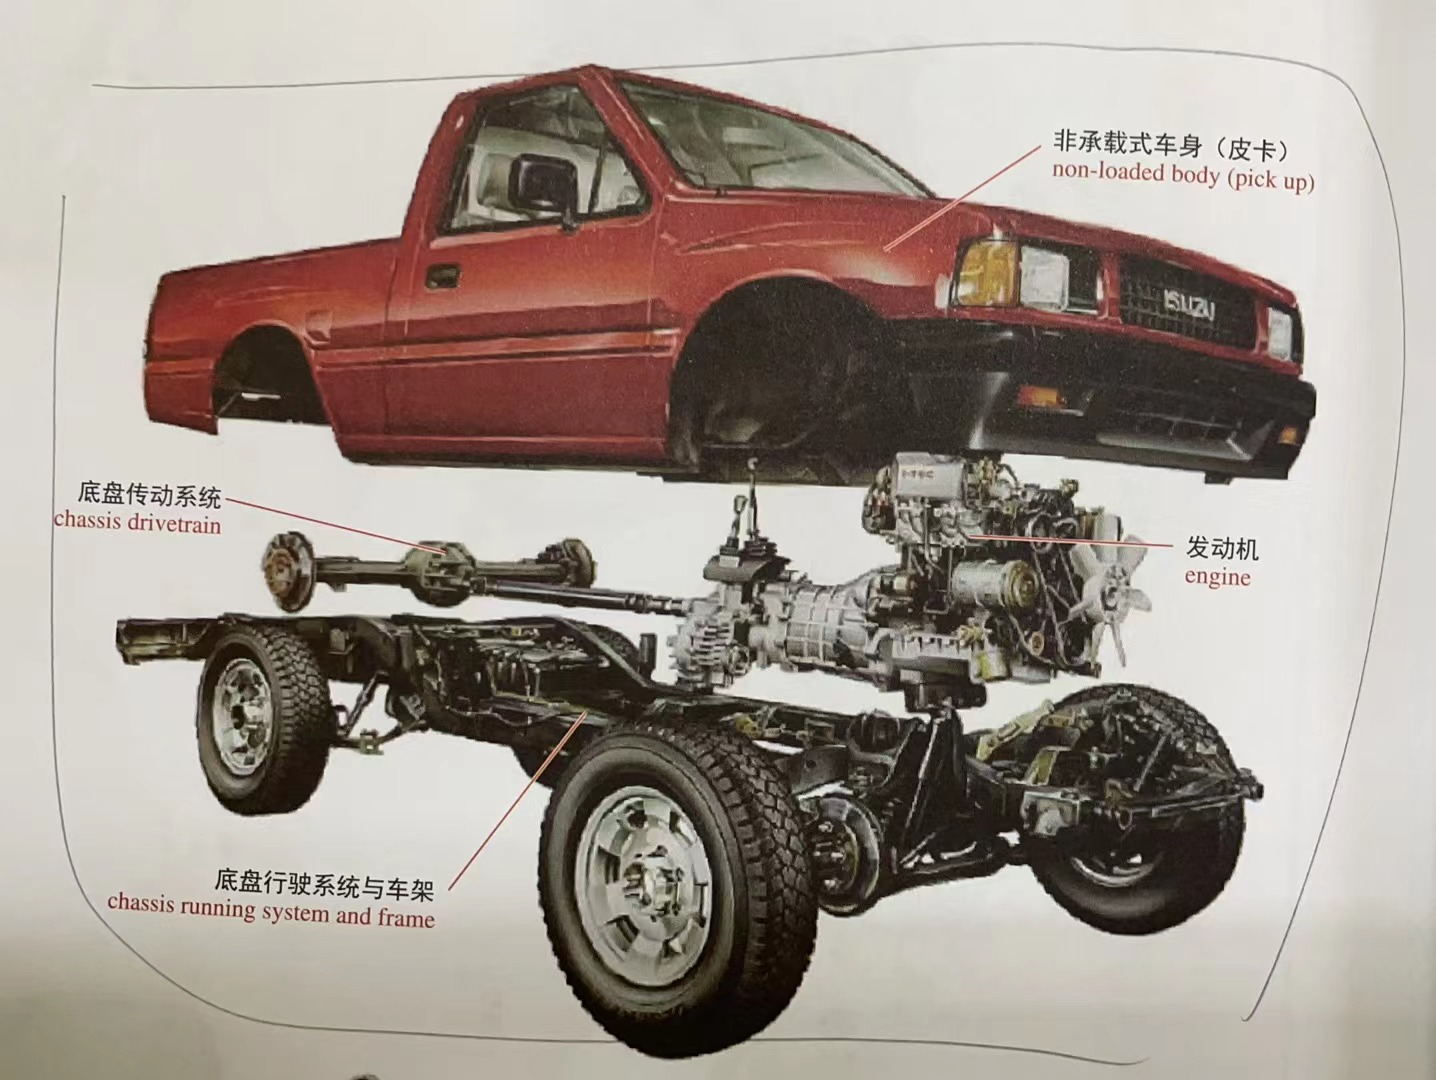
\includegraphics[width=0.5\textwidth]{4-1}
					\end{figure}
			\end{itemize}
		\clearpage
		\item 承载式车身
			\begin{itemize}
				\item  装备承载式车身的车辆没有独立的车架,车架的功能被整合到车身上
				
				\item  质量小、高度低,现代汽车普遍采用承载式车身
			\end{itemize}
			\begin{figure}[htbp]
				\centering
				\caption*{车身及底盘}
				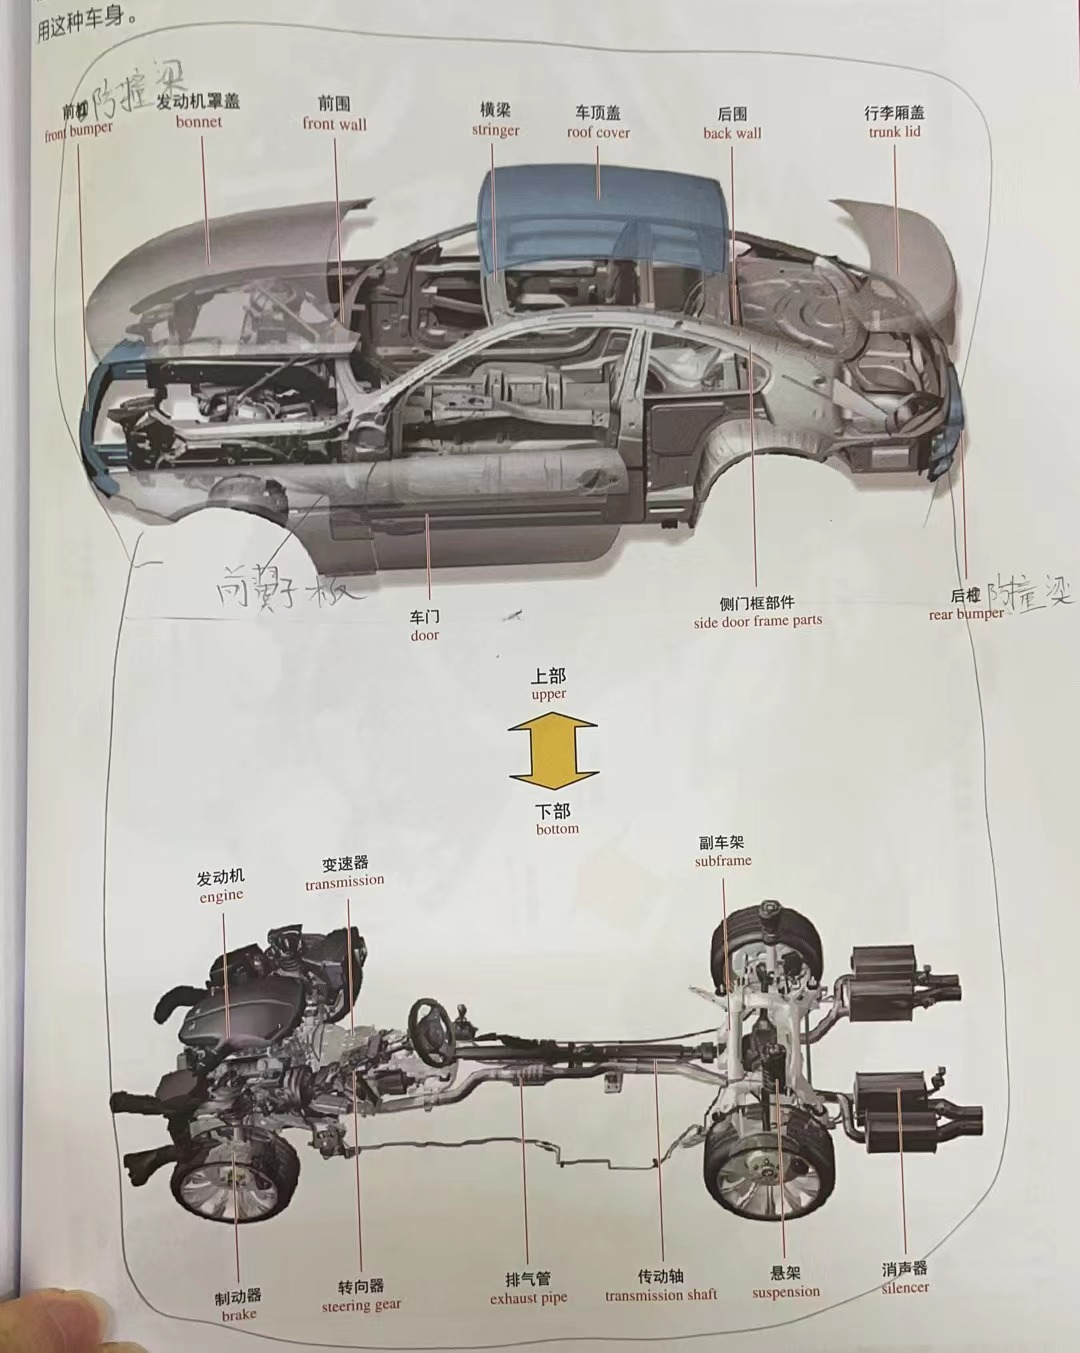
\includegraphics[width=0.6\textwidth]{4-2}
			\end{figure}
	\end{itemize}
\subsection{白车身}
车身结构件和覆盖件焊接总成

\begin{figure}[htbp]
	\centering
	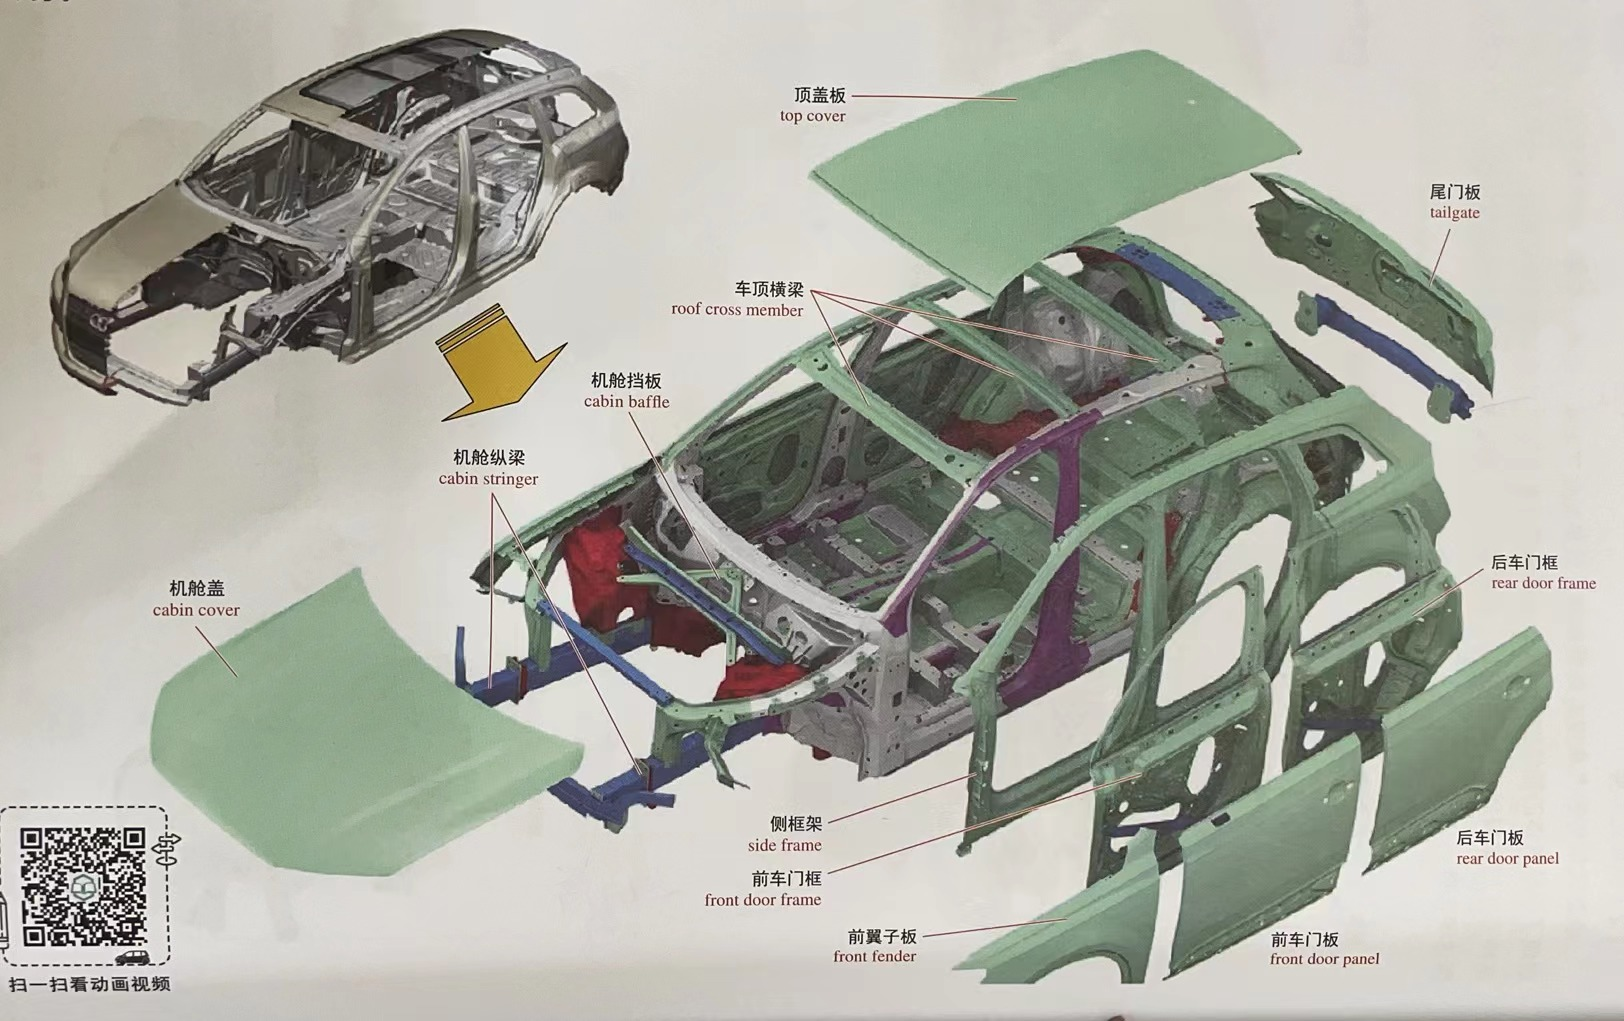
\includegraphics[width=0.5\textwidth]{4-3}
\end{figure}

\subsection{车身材料}
主要材料是钢。处于节能和环保的需求,使用较轻的材料如铝合金、镁、碳纤维增强复合材料(CFK)

钢是含碳量最高为2.06%的铁碳合金,含碳量过高为铸铁

\begin{figure}[htbp]
	\centering
	\caption{常用钢}
	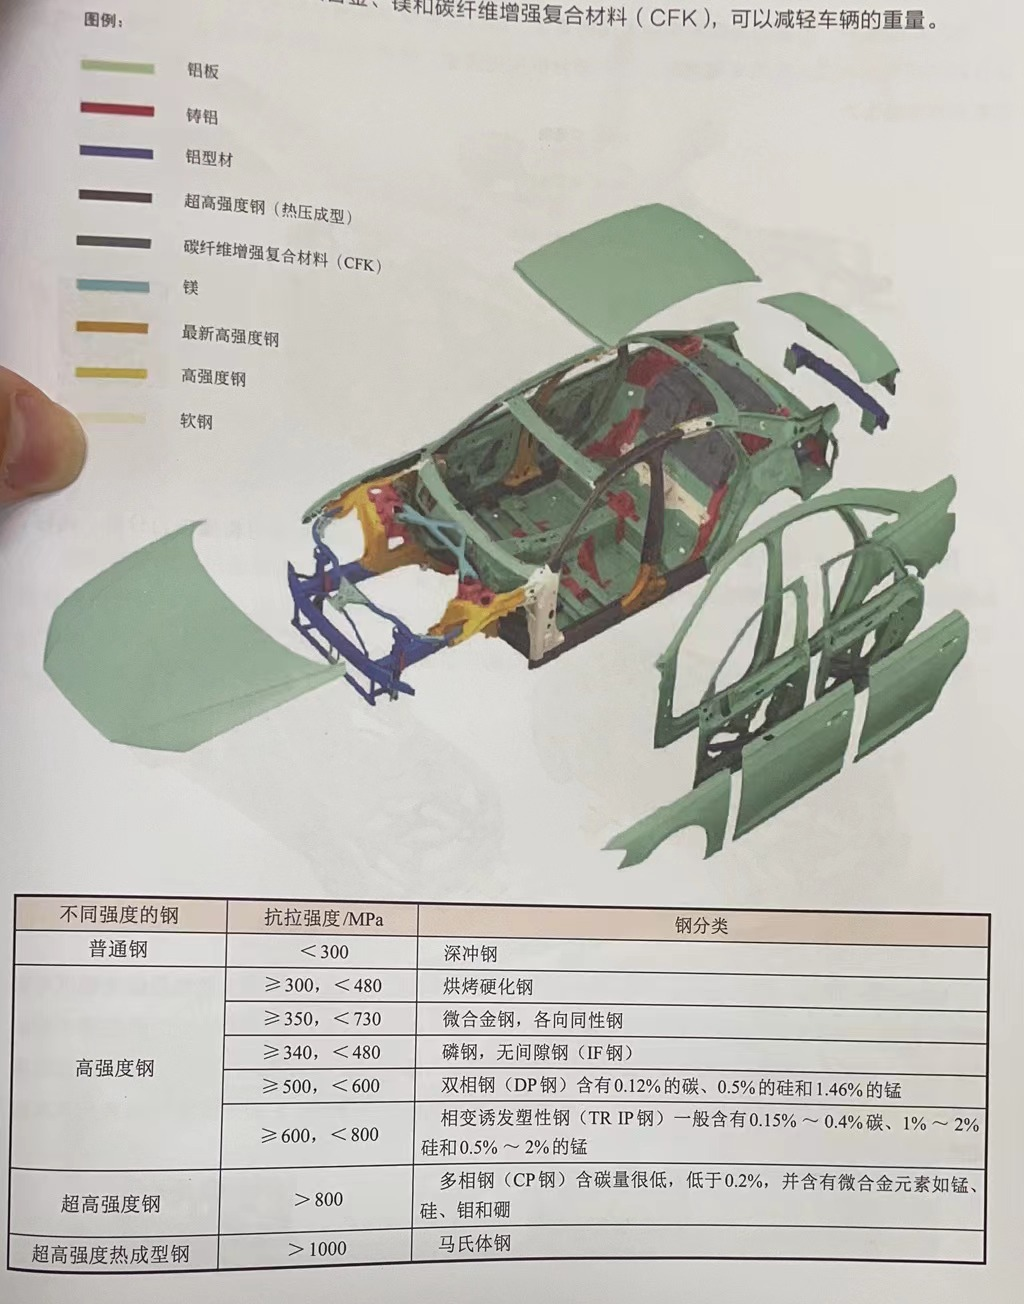
\includegraphics[width=0.6\textwidth]{4-4}
\end{figure}

\section{安全系统}
NCAP(new car assessment program)新车评价规程

\clearpage
\section{车身内饰}
	\begin{figure}[htbp]
		\centering
		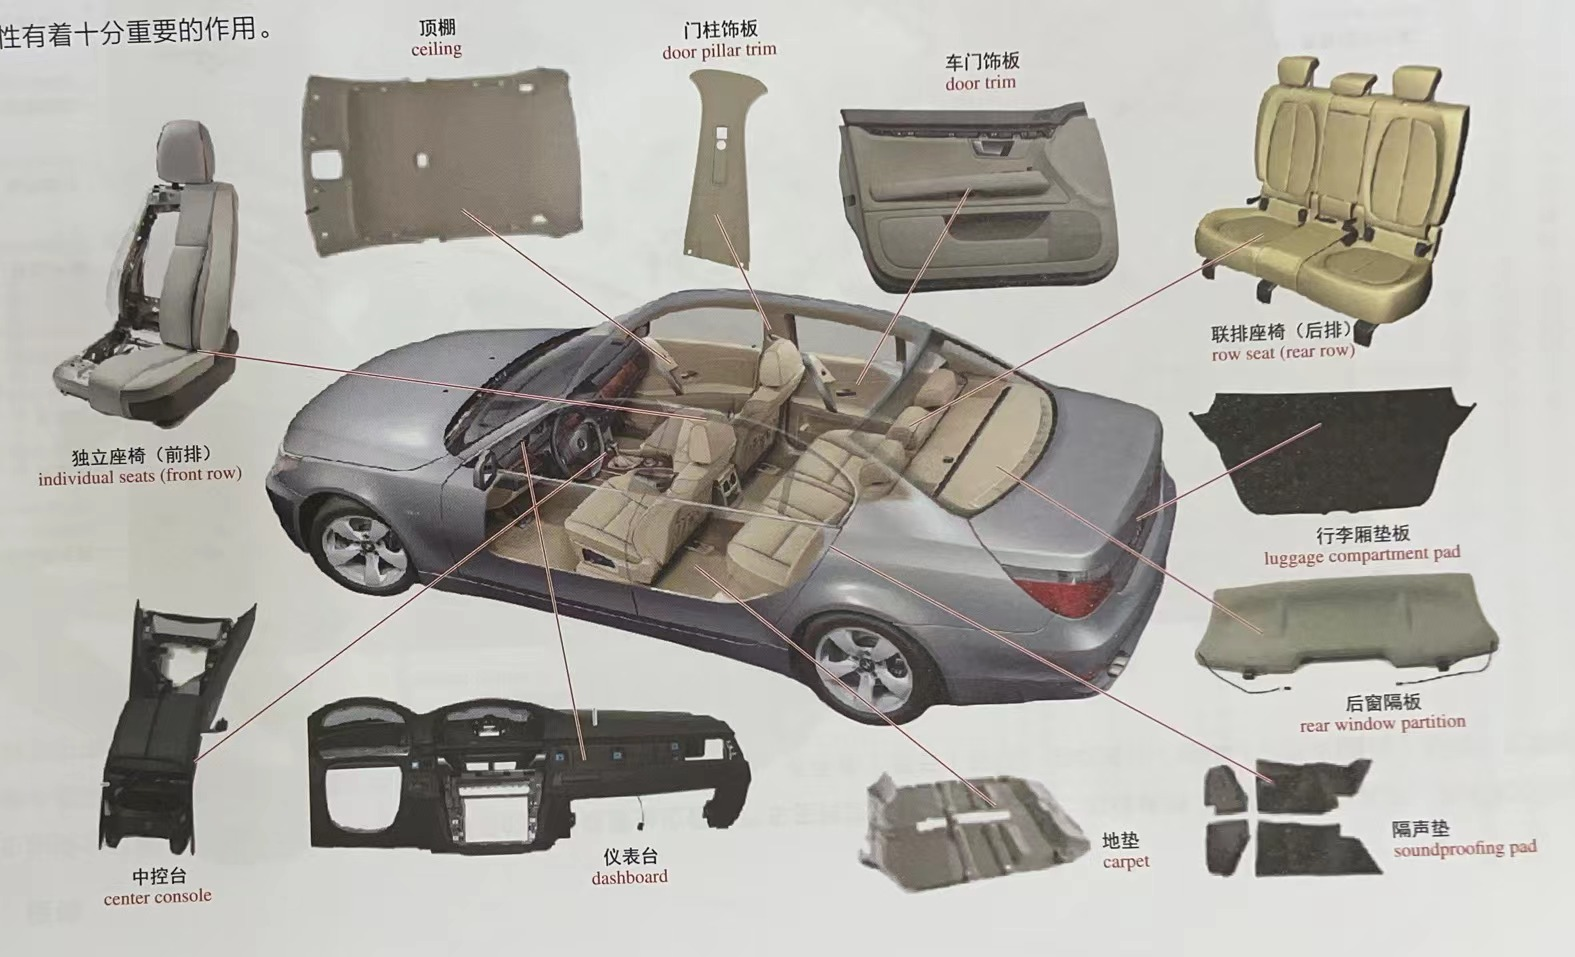
\includegraphics[width=0.5\textwidth]{4-5}
	\end{figure}
\subsection{座椅}
	按形状分:独立、联体座椅
	
	按材质分:真皮、仿革、织布座椅
	\begin{figure}[htbp]
		\centering
		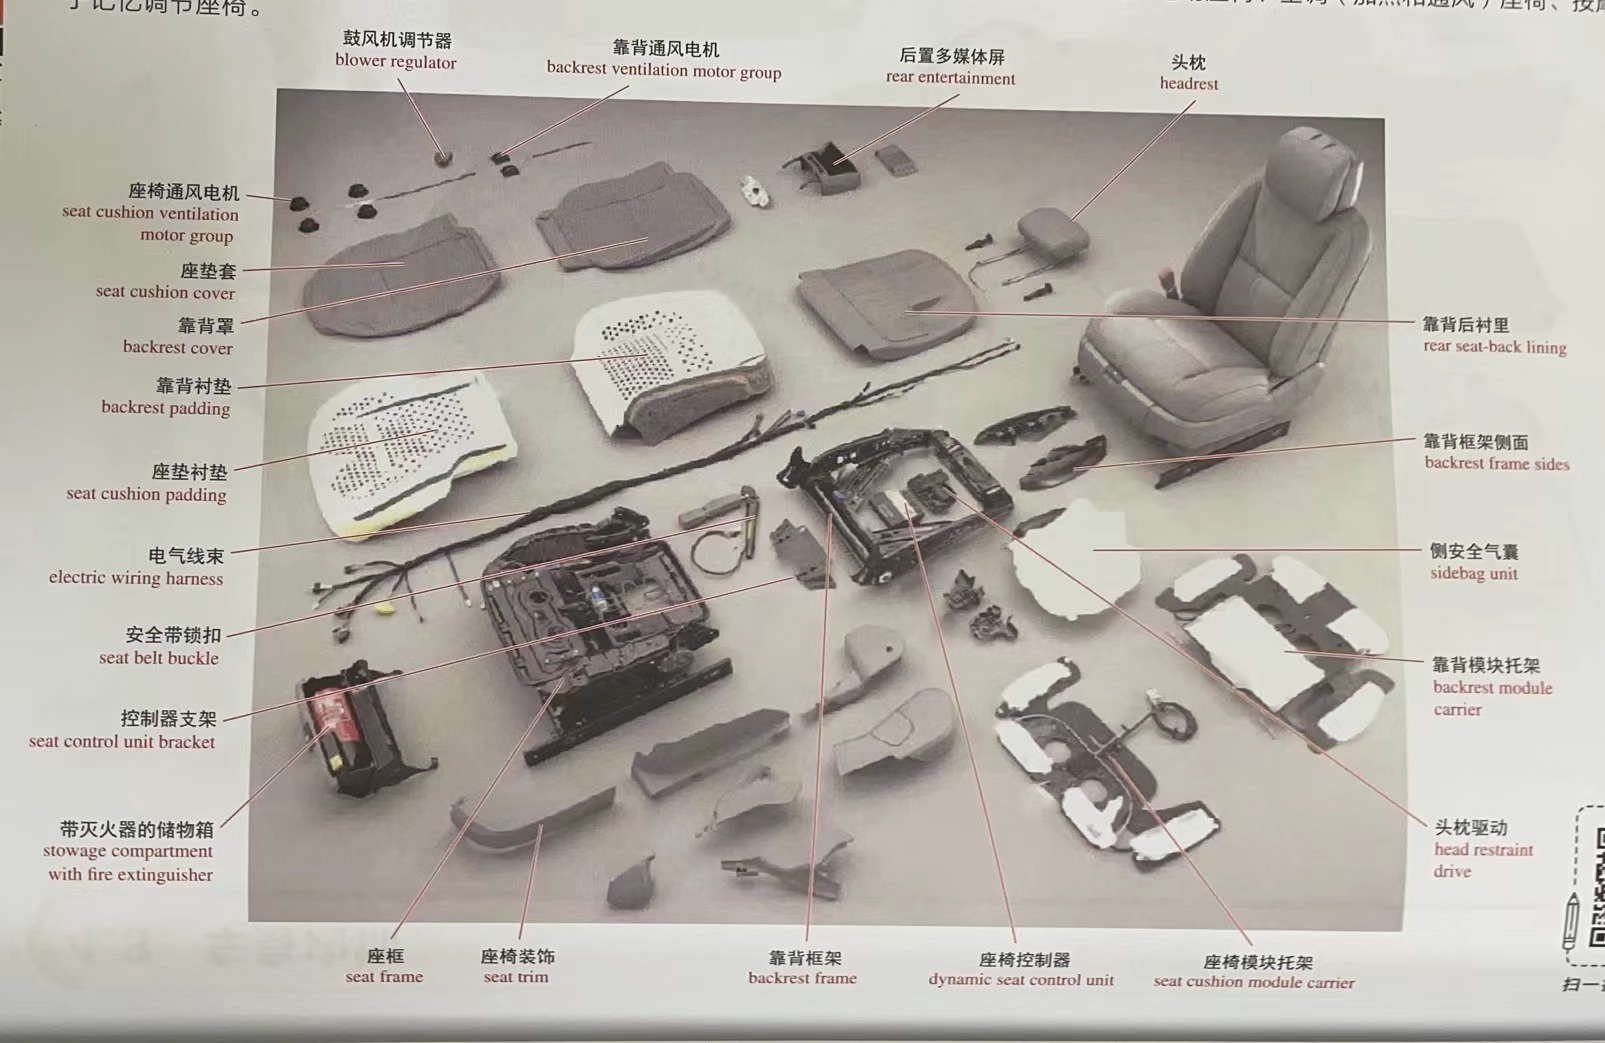
\includegraphics[width=0.5\textwidth]{4-6}
	\end{figure}
\subsection{仪表中控台}
	驾驶室中仪表和点火开关等的一个总成
	\begin{figure}[htbp]
		\centering
		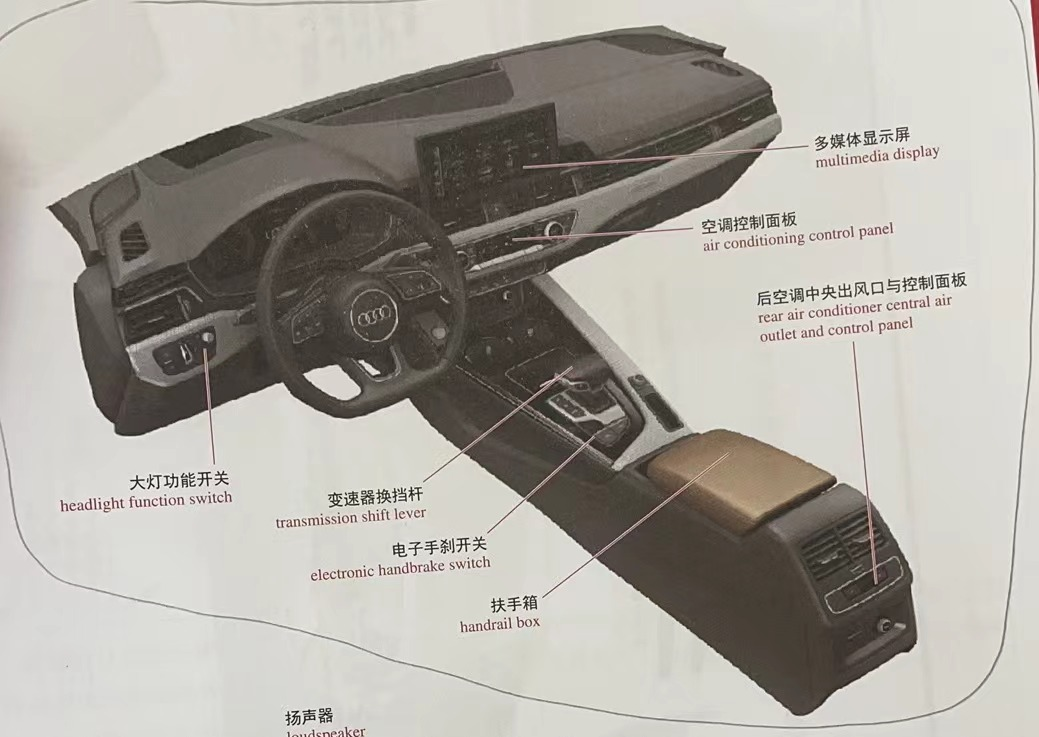
\includegraphics[width=0.35\textwidth]{4-7}
	\end{figure}
\clearpage
\section{车身外饰}

\begin{figure}[htbp]
	\centering
	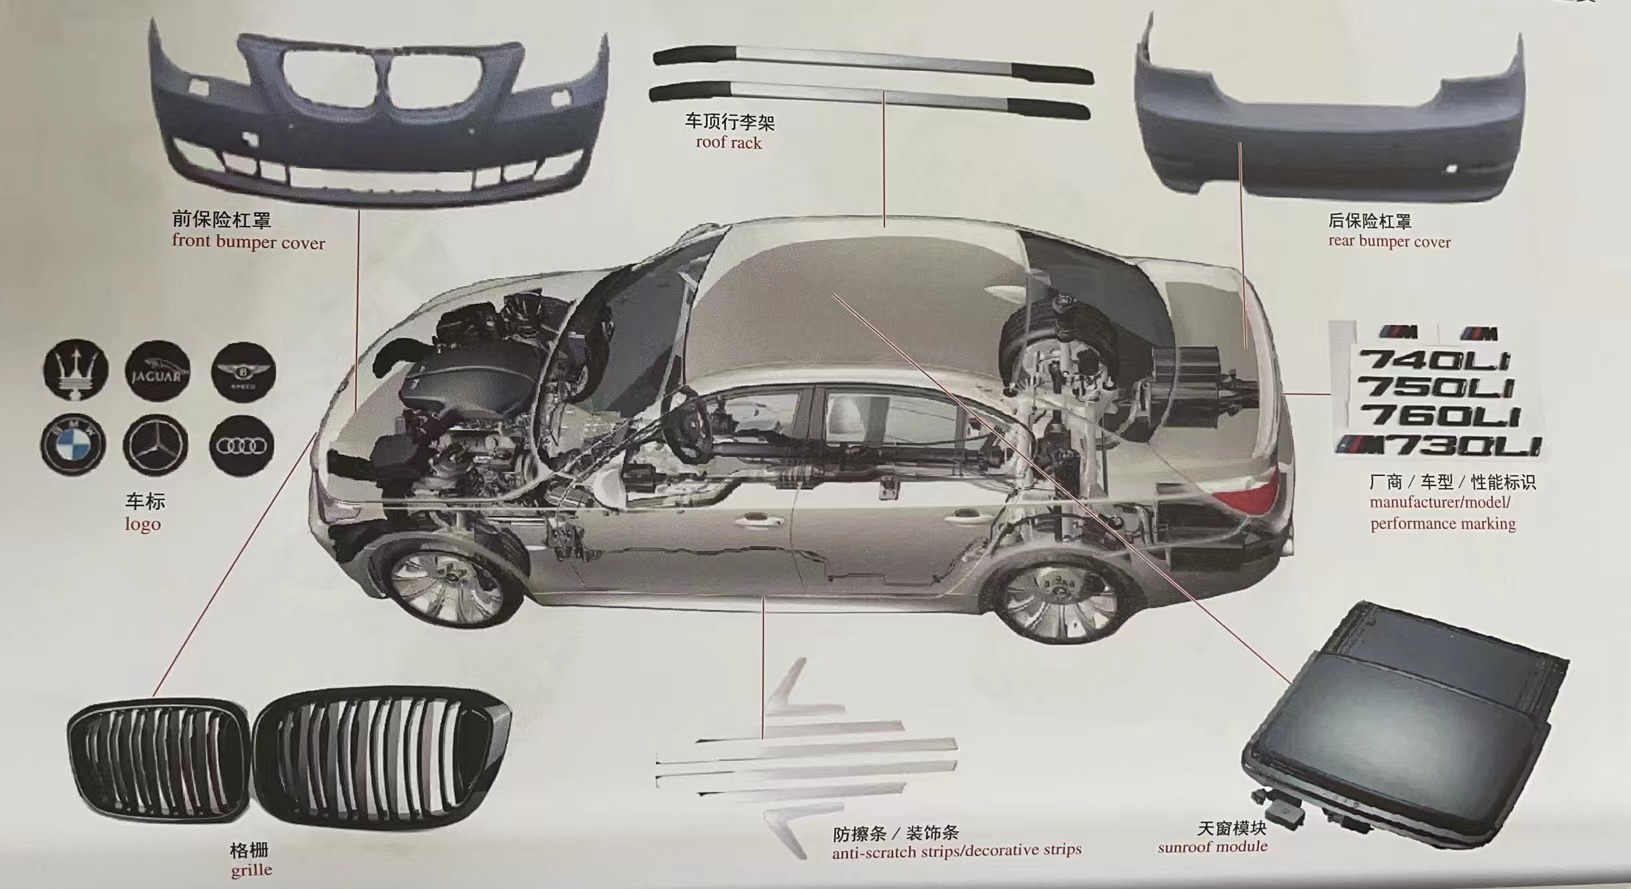
\includegraphics[width=0.5\textwidth]{4-8}
\end{figure}
\subsection{保险杠}
	保险杠一般由保险杠罩、缓冲件、防撞梁组成
	\begin{figure}[htbp]
		\centering
		\caption{前后保险杠}
		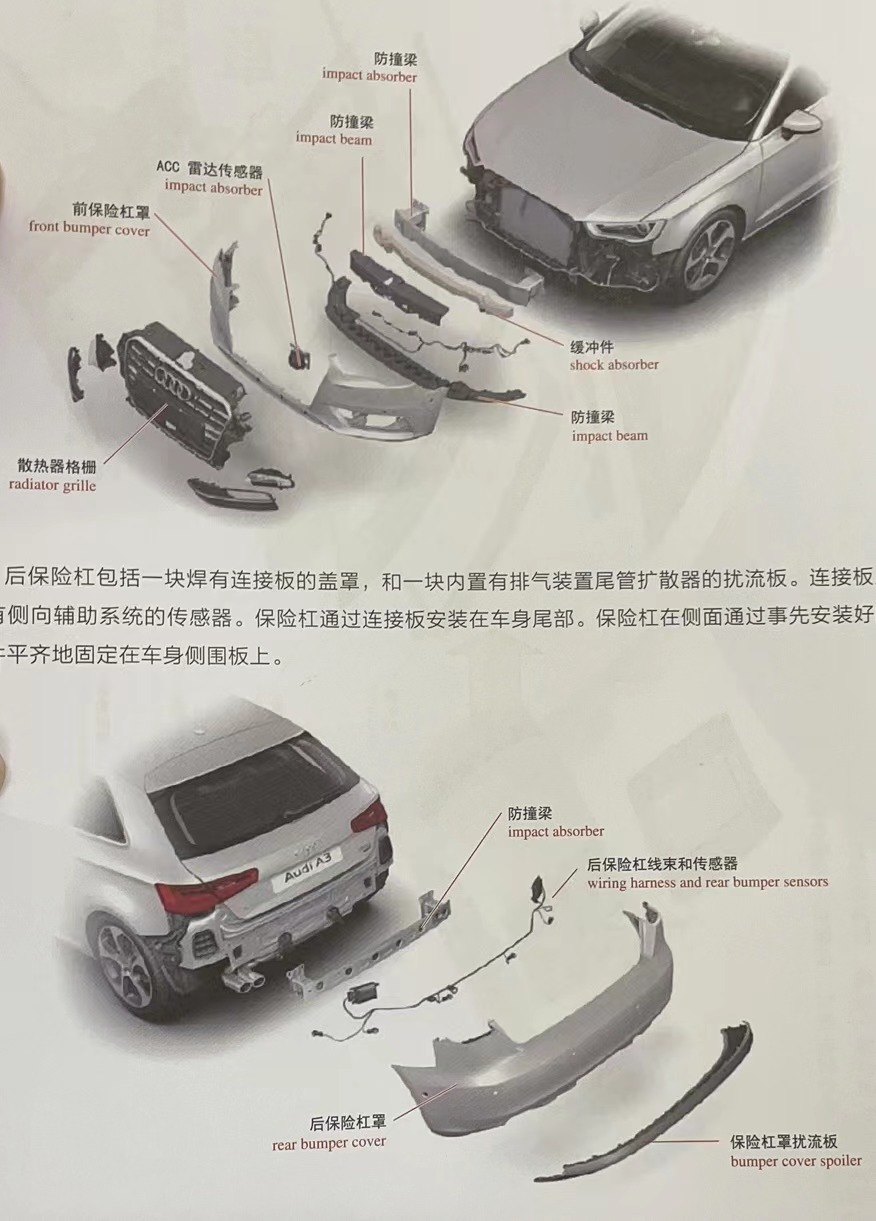
\includegraphics[width=0.35\textwidth]{4-9}
	\end{figure}

\subsection{天窗}
	\begin{figure}[htbp]
		\centering
		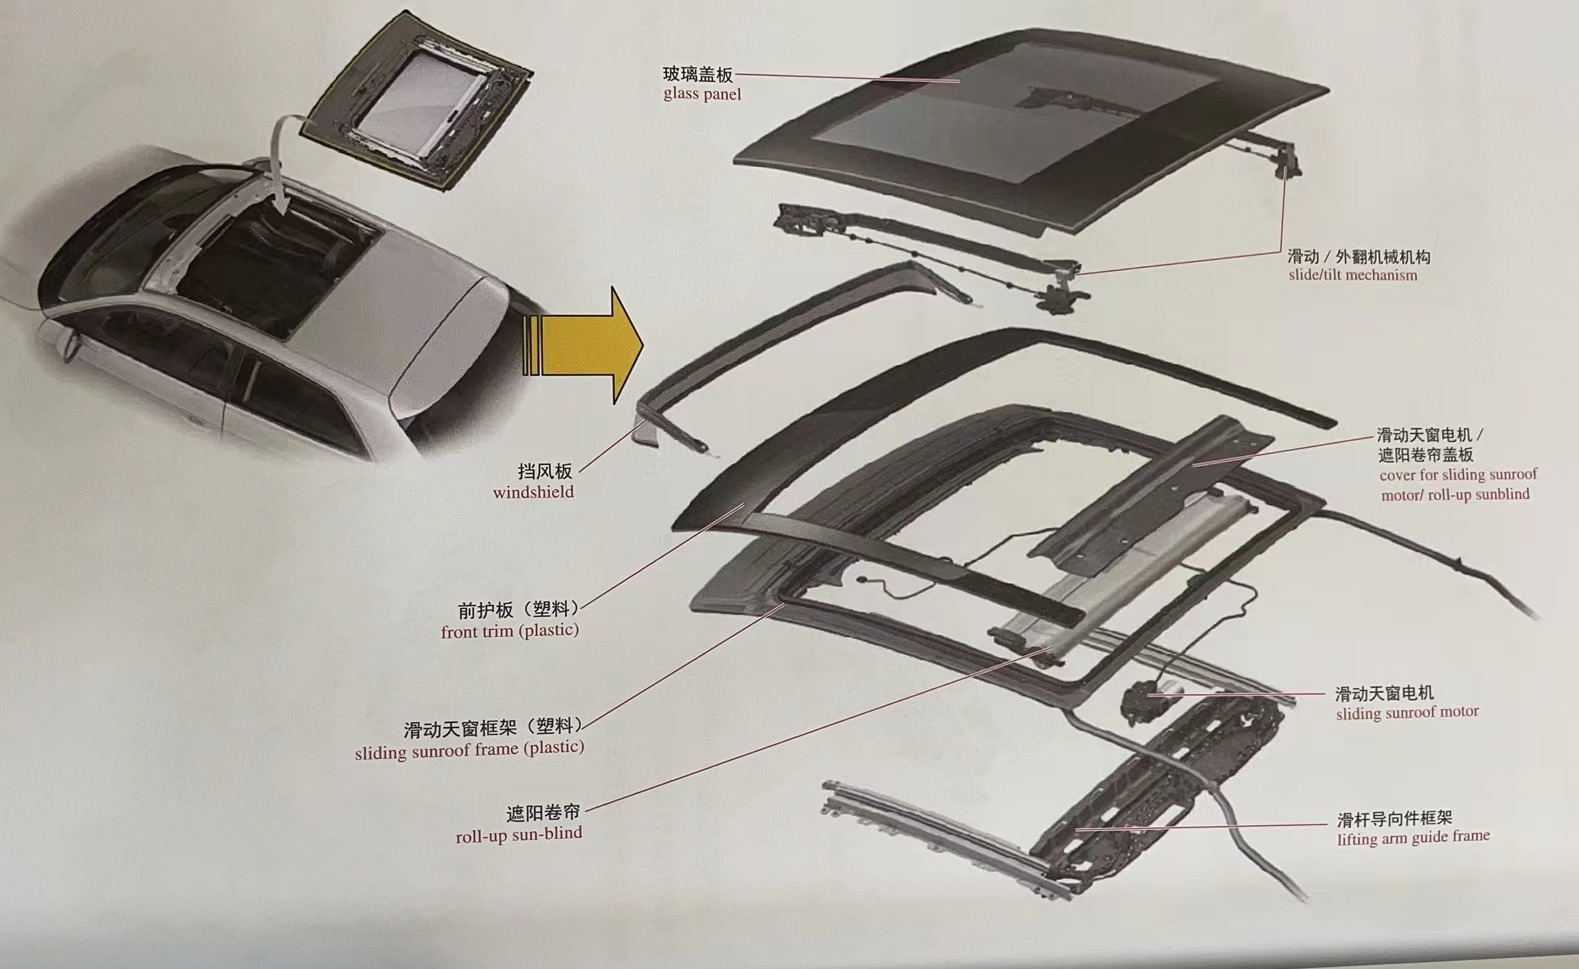
\includegraphics[width=0.46\textwidth]{4-10}
	\end{figure}
\end{document}
